\documentclass[a4paper, 12pt]{report}
\usepackage{graphicx}
\begin{document}

\title{Smarter and simple Scrabble strategy}
\date{Course: DD143X \\ Supervisor: Johan Boye \\ Kungliga Tekniska Högskolan \\ CSC \\ March 7, 2012}
\author{Frej Connolly \\ Götgatan 78 13TR LÄG1302 \\ 118 30 Stockholm \\ SWEDEN \\ +46(0)73-963 41 90 \\ connolly@kth.se \\
        \and Diana Gren \\ Sköldgatan 8 2TR \\ 118 63 Stockholm \\ SWEDEN \\ +46(0)70-467 47 20 \\ dianagr@kth.se}

\maketitle
\tableofcontents

\chapter{Introduction}
How to play a close to perfect game of Scrabble is a well studied problem. It is not as trivial as chess, checkers or tic tac toe, since there are many factors included in Scrabble that are not a part of the other classical games. For further explanations we shall introduce the expressions \emph{deterministic} and \emph{non-deterministic}. 

\begin{description}
\item[Deterministic] A game is deterministic if the players have all possible information about the state of the game, and possible future states.
\item[Non-deterministic] In contrast to a deterministic game, a non-deterministic game does not let the players now all information about the game's current or future states.
\end{description}

Unfortunately, it is not as easy to determine in which folder to put the game of Scrabble. It is not a deterministic game for sure, since we do not know which tiles are possessed by the opponent. At the same time, one could not say that it is completely non-deterministic. Imagine the end of a game, at that time all the tiles are either on the board, on the player's hand or on the opponent's hand. This results in a situation where one could figure out the complete information scope of the current state. Of course, this requires the player to know exactly how many pieces of each tile exist in the game.


\section{Problem statement}
The game require the players to have a good vocabulary and keeping an extra eye on which letter tiles that have already been placed and those who award the most points. Keeping a good balance between consonant and vocals on hand is a key to able to master the next move. It’s important to score bonus and prevent to opponent doing the same, by avoiding placing tiles that opens up a bonus square.

This gives the player many factors to take in consideration every time a move is to be made. Such factors are; words that generate higher scores, bonus tiles etc.

If there were to be a strategy where only one of these factors would be considered, which one would be the most rewarding? This study aims to investigate which of these factors has the bigger impact when one is reaching for a win. Three different programmed agents with three different objectives will play against each other in order to show results and let us determine the most preferable strategy.


\chapter{Background}

\section{Scrabble}
Scrabble was originally created by an american in the 1930s, but arrived in Sweden in 1954 according to Svenska Scrabbleförbundet \cite{forbund}. The game was renamed to Alfapet, but was named back to Scrabble after some legal issues with the game company. The game named Alfapet in Sweden still exists, but differs from the original Scrabble on some points.

The game rules are not too complicated; there can be from two up to four player playing. There is a set of tiles with letters in \emph{tha bag}, from which each player is given from 5 to 8 tiles. For consistency in the report, we say that these tiles are from the player's \emph{rack}. The objective is to form words and lay out on the board, either horizontal or vertical. The words layed out can consist of tiles from the rack, or tiles already placed on the board. The player picks up new tiles from the bag after every move.

A move can be either the player laying out a word on the board, passing his turn or changing som of the tiles on the rack for new ones from the bag. Only one of the alternatives can be made in one round. Each move generates a score, which is zero if no tiles are layed out. Otherwise, the score depends on which tiles are included in the word and also which squares of the board. The letter tiles are posessing a score number, which is higher if the letter is considered difficult to use. In addition to that, som squares on the board generates a higher score. These will be called \emph{bonus squares}. 

The last bonus opportunity is to lay out all tiles fom the rack in one move. This will give the player 50  additional points. If ont player has placed all tiles from rack, and there are no tiles left from the bag, the game ends. This will also happen if the players pass their turn four times in a row, where a pass is a move that generates zero points. 

All players that have some remaining tiles on the rack will get a penalty, which counts up to the values of the tiles left. The penalty will be drawn of the total score, and the winner of the game is naturally the player with the highest score in the end.

\subsection{Computer agents}
\section{Research}
As mentioned above, this is a well studied problem, and many papers and articles are to be found where different problems in the game of Scrabble have been studied. This paper will mostly refer to Appel and Jacobsen \cite{fastest} who discovered a way to represent the dictionary wo that it takes up minimum space in memory.
\begin{figure}
\centering
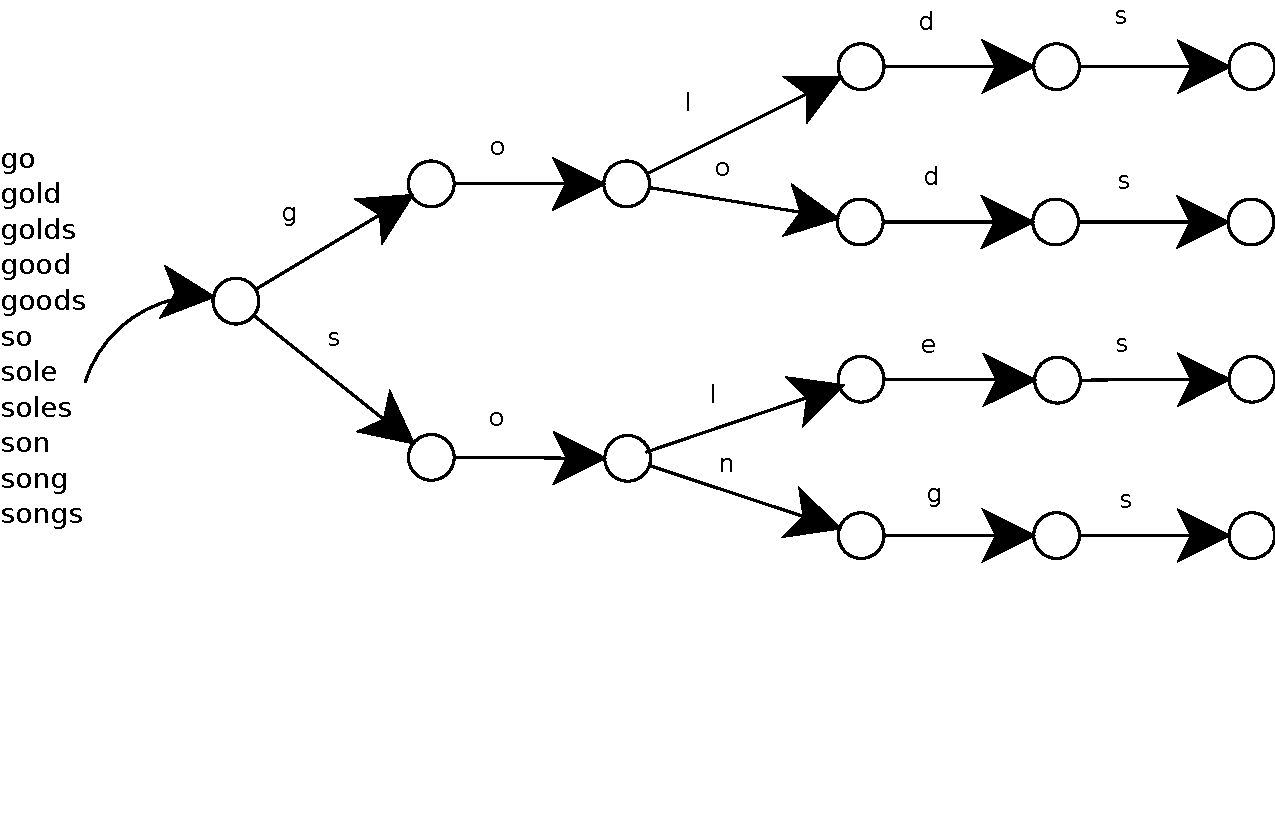
\includegraphics[scale=0.5]{trie}
\caption{Trie. Small dictionary consisting of 11 words represented as a trie.}
\end{figure}
\subsection{Dictionary}
Appel and Jacobsen \cite{fastest} came to the conclusion that a word search will be incredibly fast in a \emph{Directed Acyclic Word Graph}, which in this study will be referred to as a \emph{DAWG}. A DAWG is generally built from a trie, and can be explaind like a minimized trie. Where a trie has a lot of redundancy, becuase of edges and nodes being identical, no such thing occurres in a DAWG. All the identical edges and nodes are removed, and reduced to only one occurancy. 


\subsection{Word generation}
The problem of generating legal moves can be reduces to one dimension. Instead of doing a search in two directions (up and right) it is possible to use an algorithm that generates words only horizontally. The argument is that generating a word vertically is basically the same thing as generating a word horizontally. The only difference is that the board is transposed. Therefore, the algorithm to generate words is limited to only generate horizontally, and for each move we do two searches, where one is over the transposed board.

\subsubsection{Anchor squares}
A key in the algorithm implemented are the \emph{anchor squares}, which are the empy squares next to a non-empty square. These are important since words can only be built from already existing tiles. In the very forst move there is only one anchor; the center square, since the player making the first move always has to start in the center square.

\begin{figure}
\centering
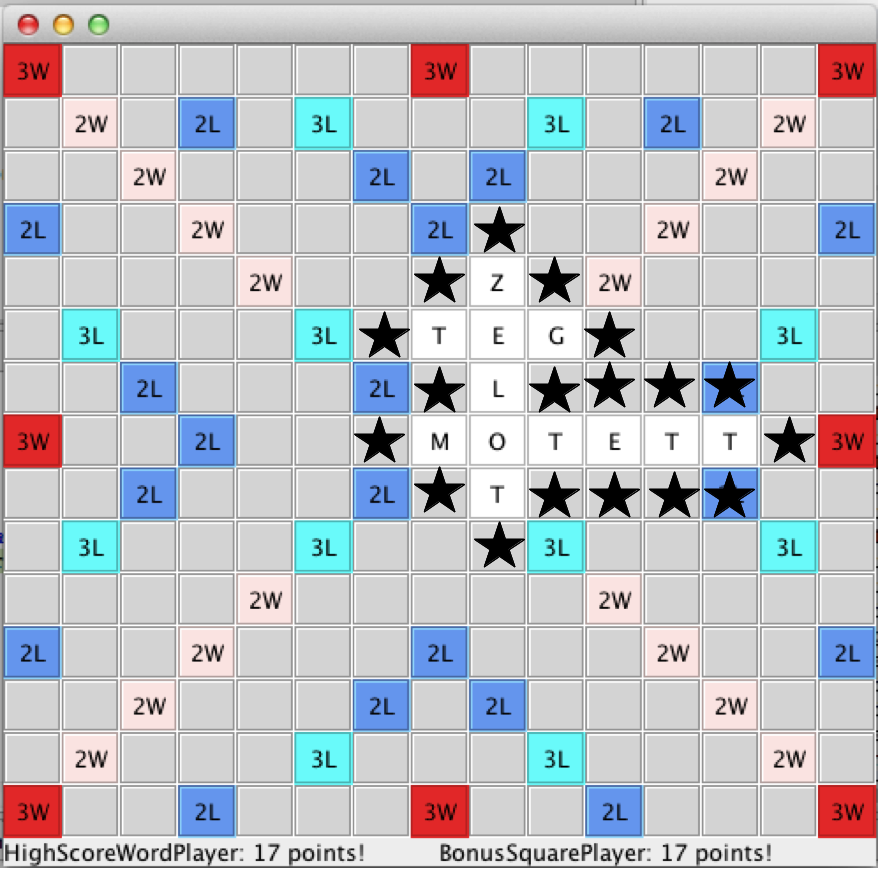
\includegraphics[scale=0.5]{anchors}
\caption{Anchor squares. The adjacent tiles are the anchor tiles from which the word generation begins.}
\end{figure}

\subsubsection{Cross-check sets}
When placing a word horizontally, the vertically placed letters also have to create a legal word. It is quite easy to establish that if we place a word horizontally, the vertical word can increas with only one letter at a time. This makes it possible to calculate, for each anchor square, which set of letters that are possible to place at that square. The calculations can be made before each move, and allows the player to place a word by row, without considering the rest of the board. The set of available letter for one square is in Appel and Jacobsen's paper \cite{fastest} referred to as a \emph{cross-check set}

\subsection{Game strategies}

\chapter{Implementation}
The study is based on an implementation that follows the example of Appel and Jacobsen \cite{fastes}, with some small modifications. Since implementing a DAWG seemed like a time consuming project, a chioce was made to stay with the trie. The advantage with a DAWG is that it saves a lot of memory, but there were no problems with memory space, and therefore an unnecessary thing to focus on.

\section{Game limitations}
There were also some restrictions made to the game, since not all rules are taken into consideration. The reason was to simplify the project and limit the work to be reasonable within the time available. The game is teherfore reduced to being played by only two players. The players do have the opportunity to lay out a word, or pass his turn. The possibility of changing the tiles is removed. In the bag of letters we also removed all blank tiles, which means no words containing Q or W can be used.

\section{Agents}
If one is a beginner at Scrabble, one probably has to make choices on what to focus on. To see which of the very basic strategis is the most successful one against the others, three agents with different strategies were implemented. The would play against each other in order to generate results for later analyze. This section describes the three different agents implemented, and their strategy in the game.

\subsection{High score words}
One strategy one can use when playing Scrabble is the fact that some letters are more worth than others. These letter are less commonly used in the language and is therefore more difficult to use. Naturally, one would want to use them as soon as there is an opportunity, to not risk getting stuck later in the game. One od the agents tested in this study follows the strategy of placing higher score generating letters first. By all legal moves generated, the agent will chose the one were the word itself has the highest score.

\subsection{Bonus tiles}
Sometimes, it can be more rewarding to place a relatively short word than a longer one. This is because of the bonus squares spread out on the board. The can multiply the value of either one letter, or the entire word placed, and can therefore generate quite high scores. The second agent strives to place words over bonus squares, to hopefully generate a high score. If there are several opportunities to reach a bonus tile, the most rewarding one is chosen by the agent, i.e. the word reaching the bonus square with the highest bonus.

\subsection{Balance on rack}
An important thing to think about when playing Scrabble is to plan for the next move. If a player ends up with only consonants on the rack, the possibility of laying out a word is reduced. The third agent tested tries to always keep a good balance between vowels and consonants on the rack, to avoid deadlocks later in the game. The agent knows the \emph{ideal ratio} and tries to lay out words so that the words left on the rack returns a ratio as close to the ideal ratio as possible. Tests with different ideal ratios are made.

\section{Test results}
\chapter{Conclusions}
\chapter{Discussion}
Naturally, the agent that only consideres a balance between tiles on the rack is not very successful. An improvement could be done to let it try to place a word with as high score as possible \emph{and} keep the balance. 

\begin{thebibliography}{100}  
  \bibitem{perfectgame} Sheppard, B., 2002, Towards Perfect Play of Scrabble, Maastricht.
  \bibitem{fastest} Appel A. W., Jacobson, G. J., 1985, The World’s Fastest Scrabble Program, Commun. ACM, 31(5), 572-585, May 1988.
\bibitem{faster} Gordon, S. A., 1993, A Faster Scrabble Move Generation Algorithm, Software - Practice and experience, Vol. 24(2), 219-232, February 1994.
\bibitem{quakle} Katz-Brown, J., O’Laughlin, J., Fultz, J., Liberty, M., Buddhdev, A., 2006, Quakle - open source crossword game software, http://people.csail.mit.edu/jasonkb/quackle/, 2 January 2012,  12 February 2012.
\bibitem{scrabblewiki} Wikipedia, Scrabble, http://en.wikipedia.org/wiki/Scrabble, 12 February 2012.
\bibitem{frank} Andersson, G., Ivansson, L., Frank - crossword software game, http://ivansson.org/Frank/, 22 August 2009, 12 February 2012.
\bibitem{wordfeud} Hbwares, Wordfeud, http://www.wordfeud.com, September 2010, 12 February 2012.
\bibitem{ai} Russell S., Norvig P. Artificial Intelligence: A Modern Approach 3rd ed. Prentice Hall. 2009
\bibitem{inforetrieve} Manning C. D., Raghavan P., Schütze H., Introduction to Information Retrieval, Cambridge University Press, 2008, p. 49-65.
\bibitem{forbund} Svenska Scrabbleförbundet, www.scrabbleforbundet.se.
\end{thebibliography}
\end{document}